\todo[inline]{This needs expansion}
We rely on previous works that have proved useful object shape representations via Gaussian Processs in the derivation of grasp controllers.
%%%%%%%%%%%%%%%%%%%%%%%%%%%%%%%%%%%%%%%%
\subsection{Equipment specification}
\label{sec:equipment}
\todo[inline]{Equipment list and specifics missing}
The vision  system should  be able  to provide  an initial  guess on  the object
location  and  observation  points  on  the  surface.  This  is  not  an  strict
requirement, since  one might  be completely blind  and still  recognize objects
around \citep[e.g.]{Petrovskaya2011Global}.  However, the use of  an initial set
of observation can  be done quickly using  RGBD sensors to speed  up the overall
process.

It is true that mounting the camera as the end-effector of a robot might allow a
full object scanning, but there might be  cases where this might not be possible
either  due to  reaching limitations  or  even sensing  capabilities on  reduced
spaces.

%%%%%%%%%%%%%%%%%%%%%%%%%%%%%%%%%%%%%%%%
\subsection{Assumptions}
\label{sec:limitations}
\todo[inline]{Needs rewording, expansion}

We assume that a point cloud of a segmented object is provided. However, we provide an optional pre-processing step that shows a reasonably way to do it when the object model is unkown.

Workspace. This is not to be thought as the workspace of a robot, but of the strategy algorithm that works on top of the object shape model. That is, we assume that we are modelling and exploring household objects that can be grasped and manipulated using a human-sized hand. This is specially useful in cases where the predicted shape is not bounded using the given observations, so this workspace will shrink the predicted shape to prevent the robot from going to an empty space, or worst, hitting undesirebly. 

We consider contact to appear when the force torque sensor measures a value higher than $1$N. The robot motion is set slow such that inertial forces are not reflected on the measurements. This is done for safety reasons, since in the phase when the robot is approaching, there is a stop signal if this threshold is superated.

%%%%%%%%%%%%%%%%%%%%%%%%%%%%%%%%%%%%%%%%
\subsection{Problem statement}
\label{sec:problem}
\todo[inline]{Needs more elaborate explanations}

Considering the equipment limitations~\ref{sec:equipment} and the assumptions~\ref{sec:limitations}, the problem for which we propose a solution can be stated as:

Given a point cloud of an object, $\mathcal{O}$, find a suitable represention for the shape that can be exploited for tasks such as object identification and grasping, and a coherent strategy to improve the representation independent of external references, i.e. intrinsic or exploiting the representation, and flexible enough to generate different exploratory actions such as poking points and sliding paths.

Many robotics applications suffer of the lack of complexity in the model used to represent the problem at hand. A new trend in robotics is to encode states and observations in a probabilistic framework to cope with novelty in the face of uncertainty. Our work follows such an approach in the sense that we integrate, in an online fashion, multi-sensory inputs (here vision and tactile clues) in a stochastic model.

This section formulates the problem of shape modelling of unknown objects (starting from a visual clue) while simultaneously planning information-gathering actions to complete our knowledge of the object to manipulate. By unknown objects, we mean that the robot does not have priory knowledge of the geometrical features of the object to be explored.  This section proceeds as follows: we first introduce a compact framework for shape estimation, here a Gaussian Process (GP), and we show how to extend such framework to estimate implicit surfaces and its first-order quantities (surface normals). Secondly, we introduce how to use such a first-order information to build an affine space of the object's surface, this procedure is called in topology as Atlas, and we also present how to exploit the affine space to compute more robust (tactile) exploration strategies in the face of shape uncertainty. 

%%%%%%%%%%%%%%%%%%%%%%%%%%%%%%%%%%%%%%%%
\subsection{Gaussian Process Regression for Implicit Surfaces}
\label{sec:gpr}
%A Gaussian Process (GP) is a (finite) collection of random variables with a joint Gaussian distribution. 

\todo[]{There's some notation conflict to fix, on later sections S is the implicit object surface.}
Let $\mathcal{S}$ be a training dataset of $N$ observations, $\mathcal{S}=\{(\mathbf{x}_i, y_i)|i=1,\dots,N\}$, where $\mathbf{x}_i\in\mathbb{R}^D$ denotes the $i^{th}$ input vectors and $y_i\in\mathbb{R}$ the associated scalar output or target.  We collect the $N$ inputs vectors in a $D\text{x}N$ matrix $X$ and the output target in a $N\text{x}1$ vector $\mathbf{y}$, so that we can rewrite the training dataset in a more compact way as $\mathcal{S}=\{(X,\mathbf{y})\}$. We are interested in making inference about the mapping function $f:\mathbb{R}^D\rightarrow\mathbb{R}$ between the input vectors and the targets. We assume a linear regression model
$$
y_i=f(\mathbf{x}_i)+\epsilon
$$
where $\epsilon\thicksim\mathcal{N}(0,\sigma_n^2)$ is an independent identically distributed Gaussian noise with zero-mean and variance $\sigma_n^2$. 

A Gaussian Process framework for regression (GPR) is a common choice to approximate $f(\mathbf{x})$, in which the targets $y_i$ are assumed to be drawn from a zero-mean multi-variate Gaussian distribution with a covariance matrix which is a function of the input vectors. Therefore the output distribution can be written as
$$
(y_1,\dots,y_N|\mathbf{x}_1,\dots,\mathbf{x}_N)\thicksim\mathcal{N}(0,K(X,X)+\sigma_n^2I)
$$
The covariance function expresses somehow the notion of nearness or similarity, for which points in the input space $\mathbb{R}^D$ that are close would likely produce similar outputs. The choice of a kernel is a crucial ingredient for a GP and a vast part of the literature has investigated this problem, sometimes referred as the \emph{kernel trick}. Following previous works on implicit surface estimations we chose the \emph{thin plate} kernel, which is defined as
\begin{eqnarray}
\label{eq:thinplate}
K(\mathbf{x}_i,\mathbf{x}_j)=2\|\mathbf{x}_i-\mathbf{x}_j\|_2^3-3R\|\mathbf{x}_i-\mathbf{x}_j\|_2^2+R^3
\end{eqnarray}
where $\|\mathbf{a}\|_2=\sqrt{\mathbf{a}^\top\mathbf{a}}$ and $R=\max(\|\mathbf{x}_i-\mathbf{x}_j\|_2),\forall\mathbf{x}_i,\mathbf{x}_j\in\mathcal{S}$, is the largest pairwise distance between the input vectors in the training dataset $\mathcal{S}$. To improve the prediction performance of the GP with a thin plate kernel is useful to divide the training dataset in three disjointed subsets, namely $\mathcal{S}^0=\{(\mathbf{x}_i,y_i)|y_i=0\}$ are the input point on the object's surface, $\mathcal{S}^+=\{(\mathbf{x}_i,y_i)|y_i=+1\}$ and $\mathcal{S}^0=\{(\mathbf{x}_i,y_i)|y_i=-1\}$ are artificial points, respectively, outside and inside the object's surface. We then can rewrite as $S=S^0\cup S^+\cup S^-$.

Given a new point $\mathbf{x}_*$, it is possible to query the GP to compute the estimate of $y_*=f(\mathbf{x}_*)+\epsilon$ with a measure of confidence expressed by the associated variance $\mathbb{V}[y_*]$ by computing the following equations:

\begin{eqnarray}
\label{eq:gpr_mu}
y_*=\mathbf{k}_*^\top(K+\sigma_n^2I)^{-1}\mathbf{y}
\end{eqnarray}

\begin{eqnarray}
\label{eq:gpr_var}
\mathbb{V}[y_*]=k(\mathbf{x}_*,\mathbf{x}_*)-\mathbf{k}_*^\top(K+\sigma_n^2I)^{-1}\mathbf{k}_*
\end{eqnarray}
we introduced a more compact notation where, for a single query point $\mathbf{x}_*\in\mathbb{R}^D$, $\mathbf{k}_*=K(\mathbf{x}_*,X)$ is the $N\text{x}1$ covariance vector between the query point and the training dataset $X$. Similarly, $K=K(X,X)$ is the covariance matrix evaluated on the training dataset and $k(\mathbf{x}_*,\mathbf{x}_*)$ is a scalar value denoting the variance between the query point and itself.
\todo[inline]{To add Gradient regression, perhaps in another subsec}

\subsection{Gaussian process derivative}

In the previous section we have introduced a general formulation of GPR for implicit surfaces in which is possible to predict new target values of $f(\mathbf{x})=0$ with their associated expected variance $\mathbb{V}[f(\mathbf{x})]$. In this section we show how to compute first-order quantities (the normals to the object's surface) directly from the GP.  Similarly to Eq.\ref{eq:gpr_mu} the expected normal on the query point $\mathbf{x}_*$ is computed as

\begin{eqnarray}
\label{eq:gpr_n}
n_*=\frac{\partial\mathbf{k}_*}{\partial\mathbf{x}}^\top(K+\sigma_n^2I)^{-1}\mathbf{y}
\end{eqnarray}

where $\frac{\partial\mathbf{k}_*}{\partial\mathbf{x}}=\frac{\partial\mathbf{k}(\mathbf{x}_*,X)}{\partial\mathbf{x}}\vert_{\mathbf{x}=\mathbf{x}_*}$

\begin{figure}[h]
    \centering
    \mbox
    {
        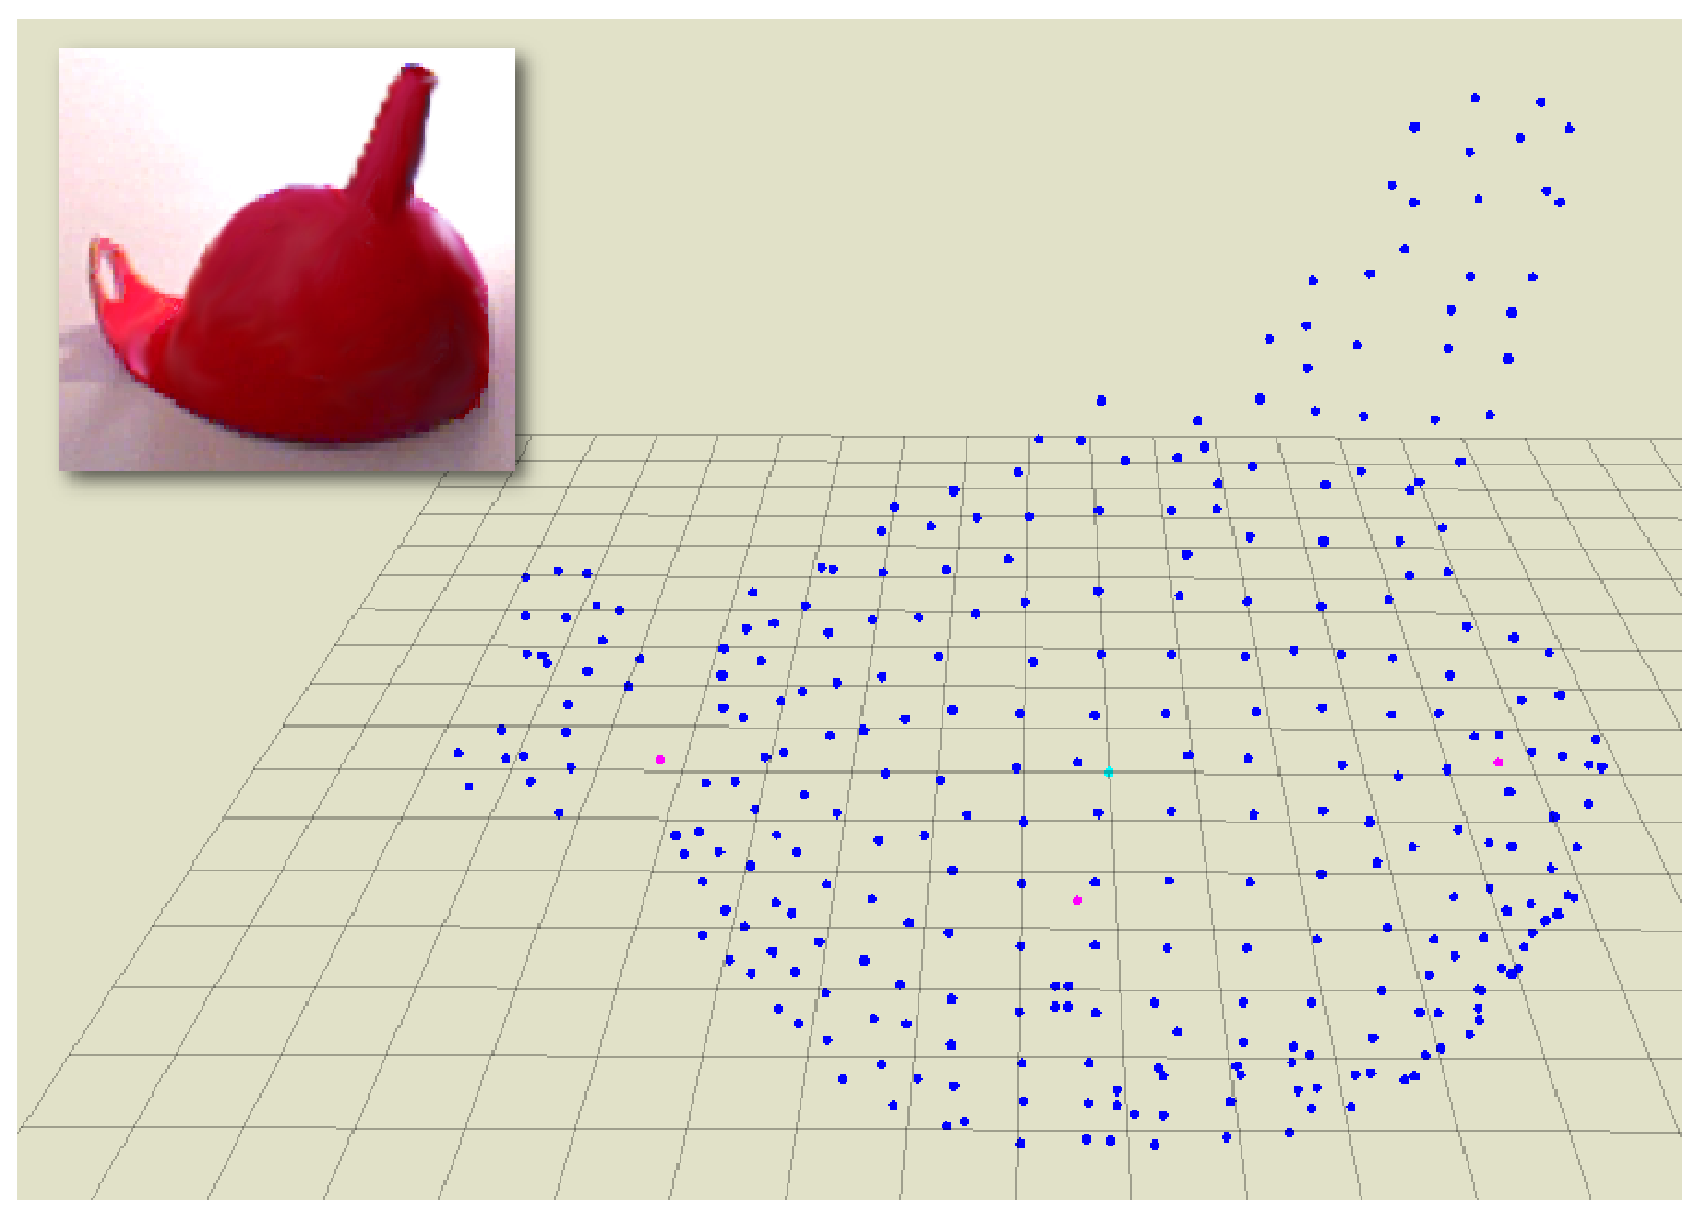
\includegraphics[width=0.45\linewidth]{funnelC.eps}
        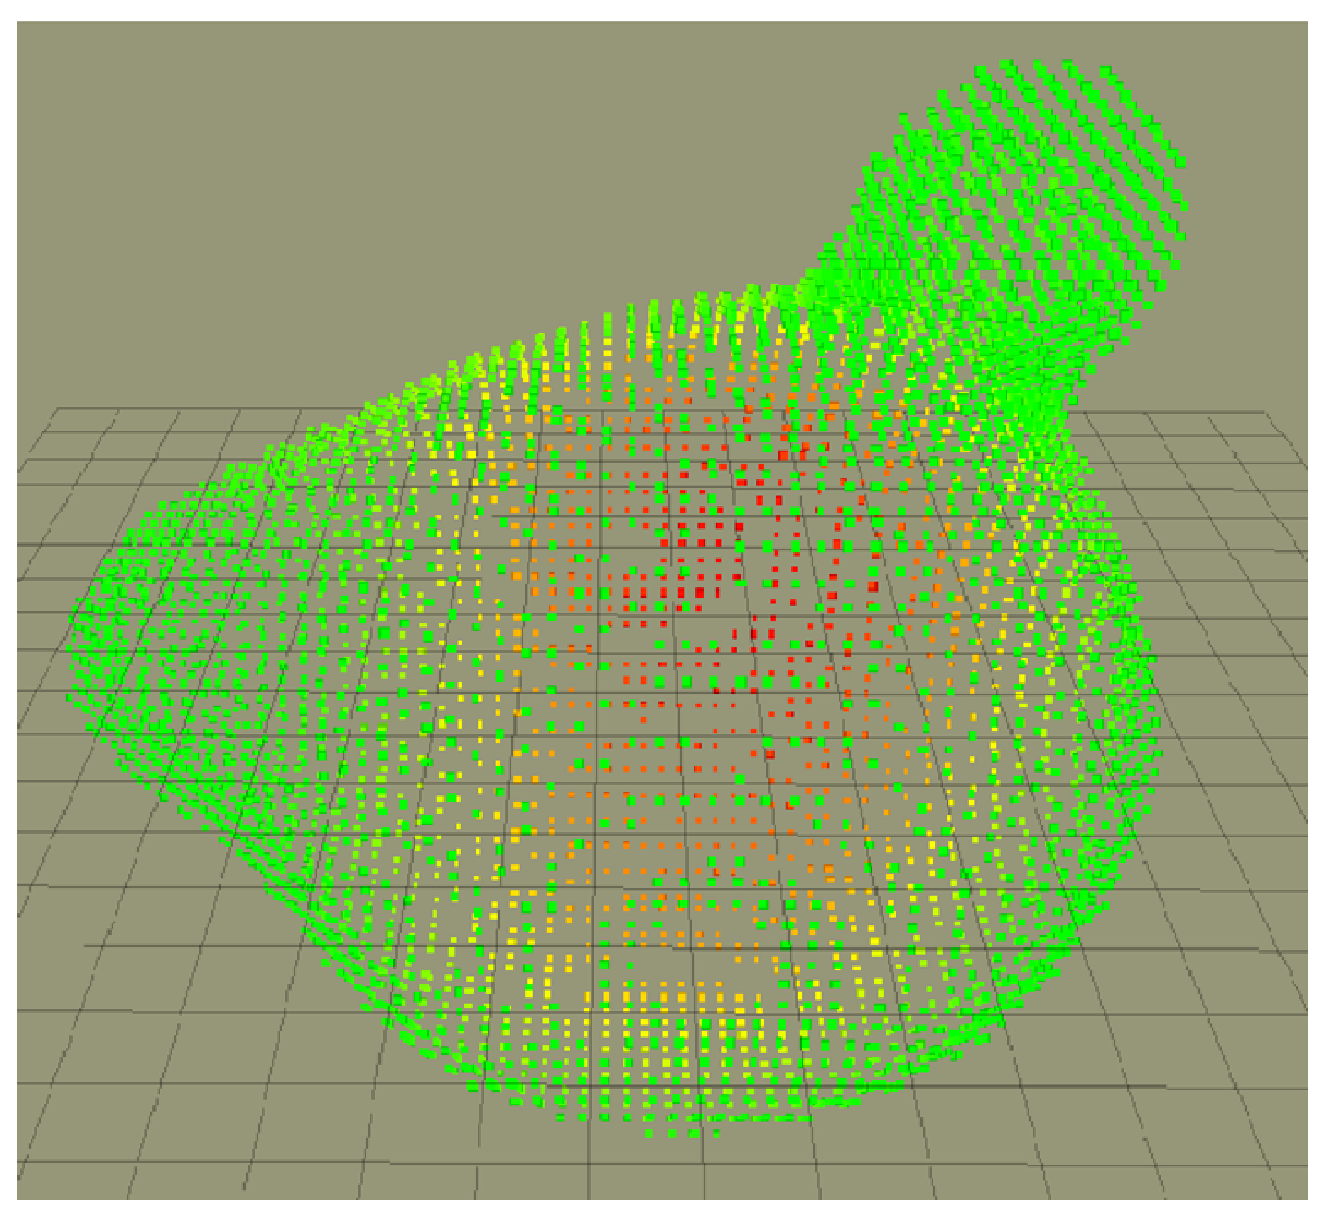
\includegraphics[width=0.45\linewidth]{funnelS.eps}
    }
    \caption{Gaussian Process regression on a funnel object. }
    \label{fig:GPfunnel}
    \todo[inline]{just added to see how it looks on the paper}
\end{figure}
\begin{figure}[h]
    \centering
    \mbox
    {
    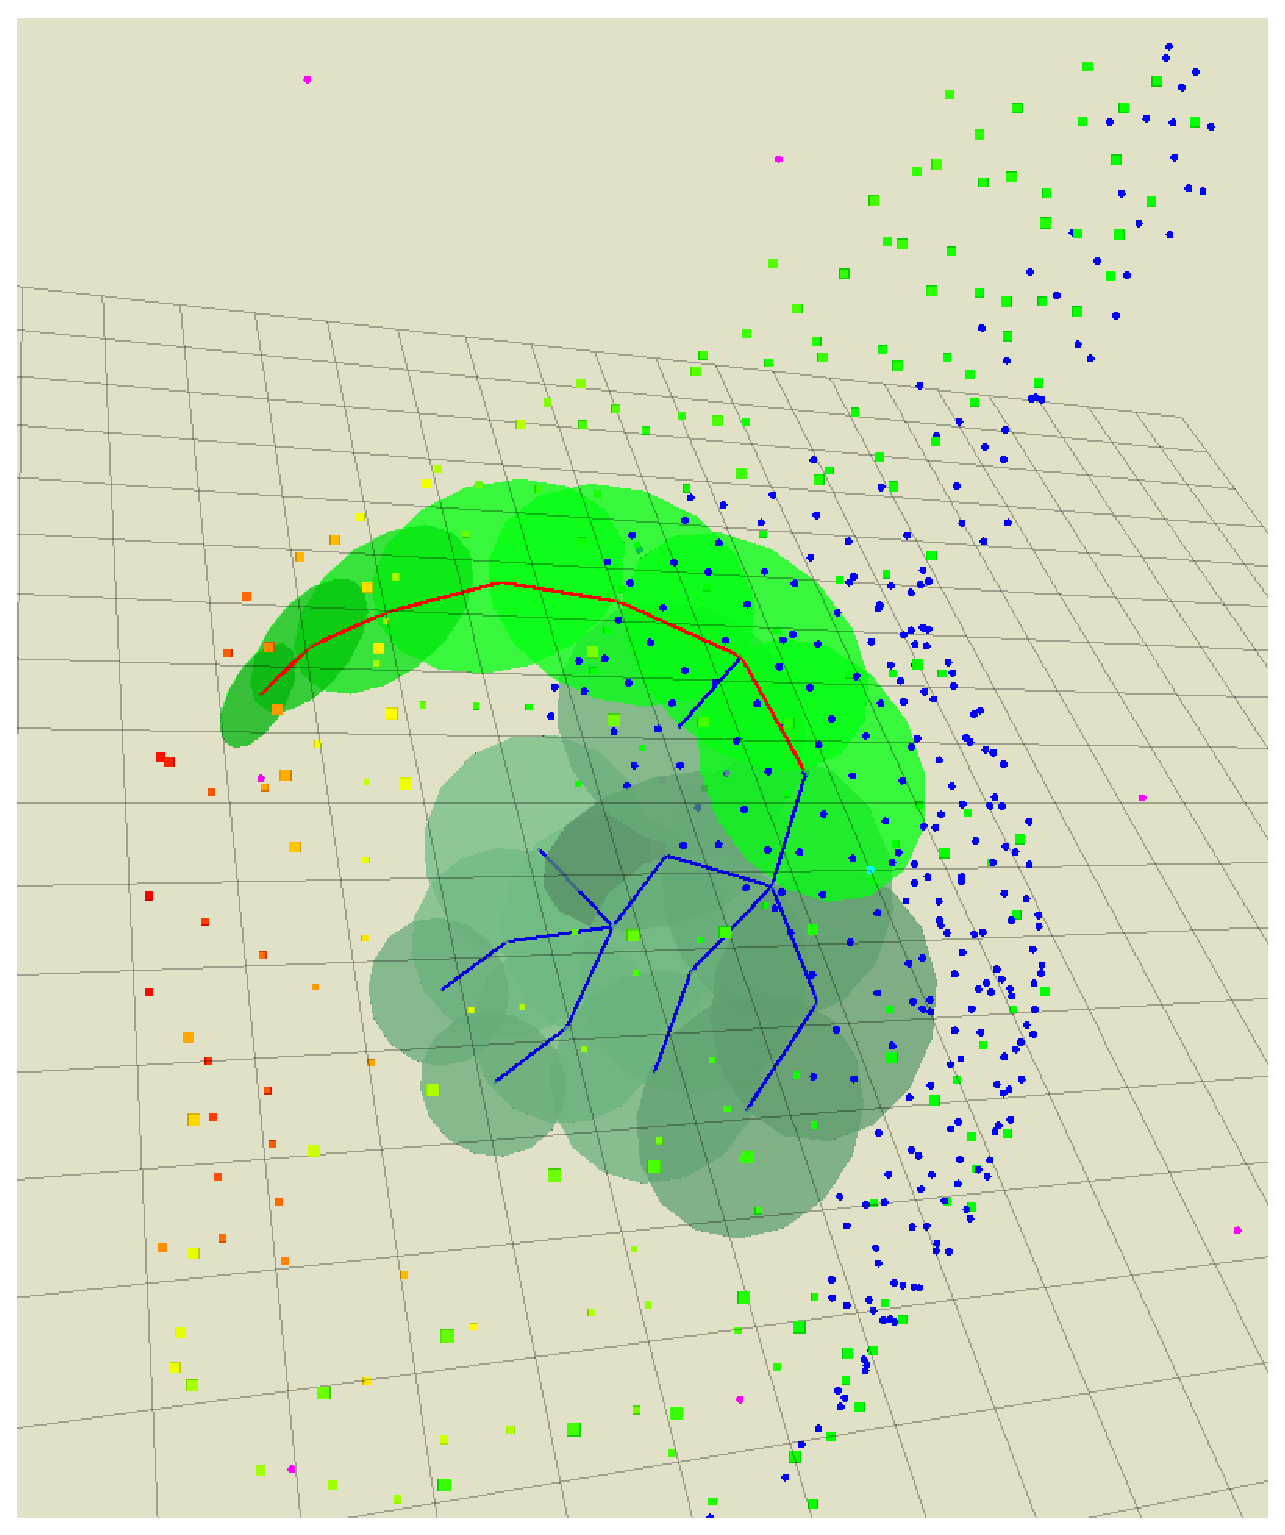
\includegraphics[width=0.45\linewidth]{funnelRRT.eps}
    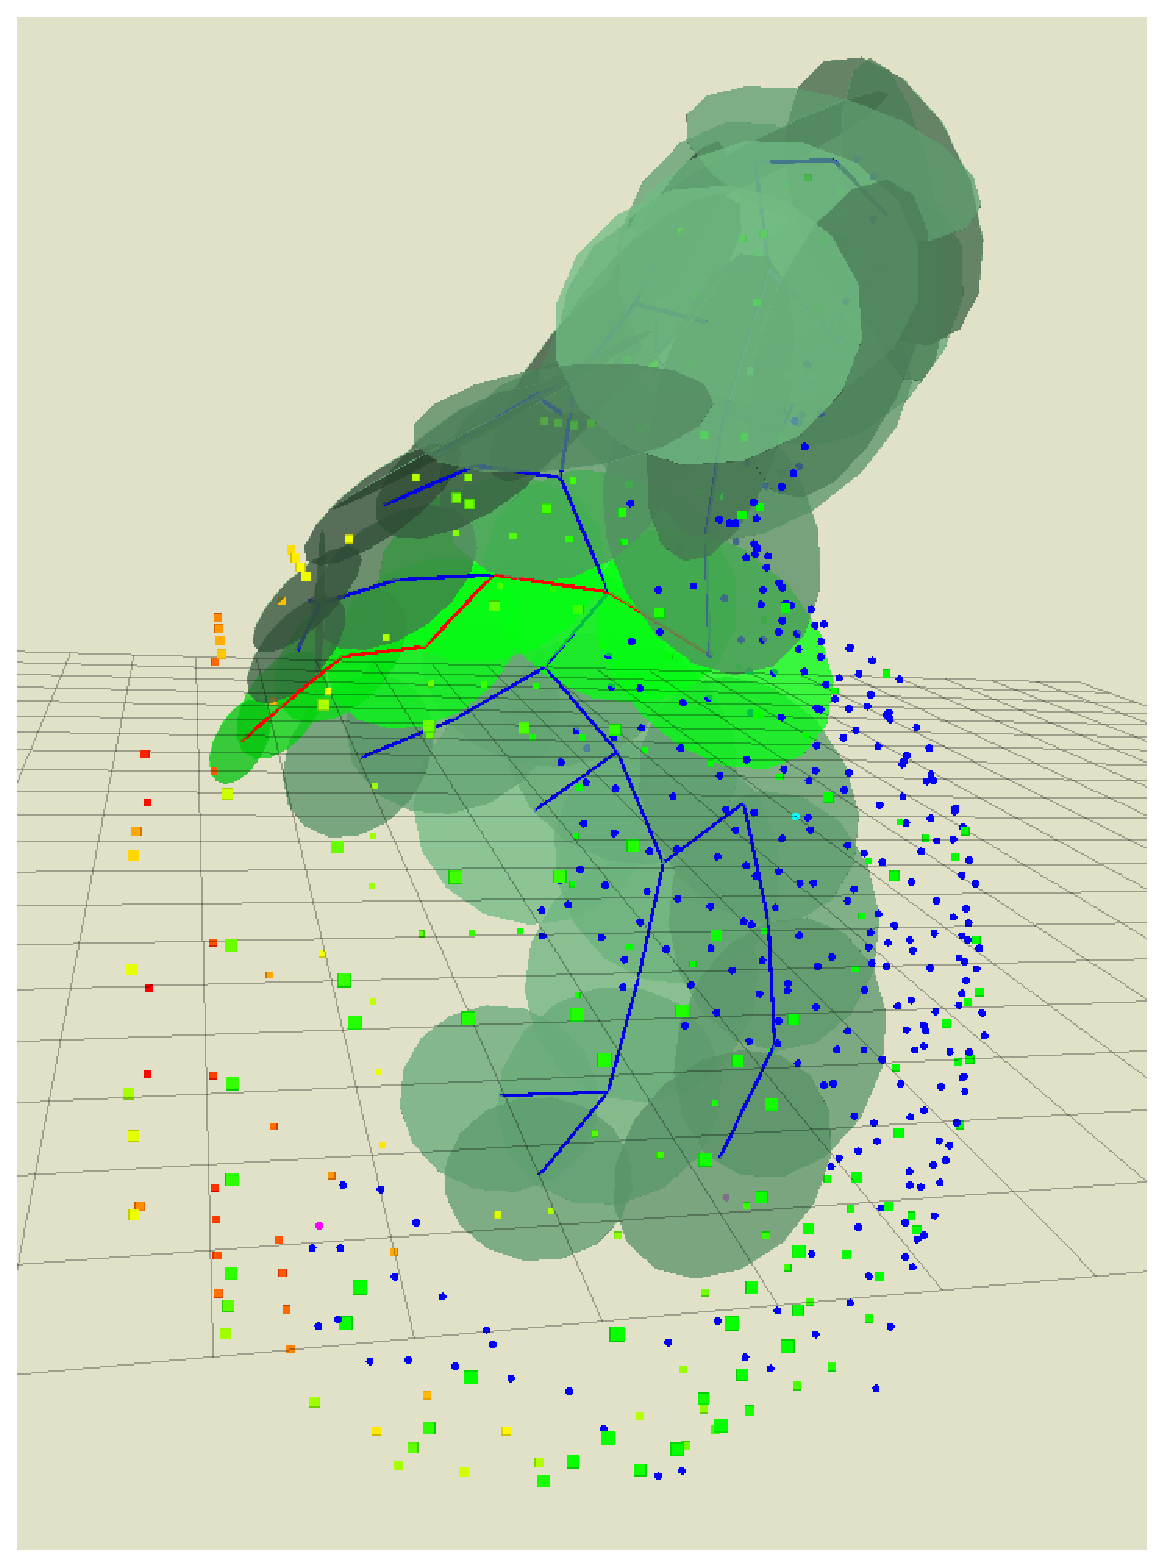
\includegraphics[width=0.45\linewidth]{funnelRRT2.eps}
    }
    \caption{RRT explorer on the funnel implicit surface. Solution is highlighted in green.}
    \label{fig:RRTfunnel}
    \todo[inline]{just added to see how it looks on the paper}
\end{figure}


























